%\documentclass[leterpaper][13pt]{article}
\documentclass{article}
\usepackage[T5]{fontenc}
\usepackage[utf8]{inputenc}
%\usepackage[vietnam]{babel}
\usepackage{hyperref}
\usepackage{amsmath}
\usepackage{graphicx}
\graphicspath{{images/}}
%\usepackage{parskip}
%\author{Linus C. Brendel}								% Author
\date{\today}											% Date
%vnd thêm vào để có thể chuyển Figure => Hình											
\renewcommand{\figurename}{Hình}
%\usepackage[labelsep=endash]{caption}

\begin{document}
%%%%%%%%%%%%%%%%%%%%%%%%%%%%%%%%%%%%%%%%%%%%%%%%%%%%%%%%%%%%%%%%%%%%%%%%%%%%%%%%%%%%%%%%%

\begin{titlepage}
	\centering
	\vspace*{0.5 cm}
	\textsc{\LARGE Báo Cáo Kết Thúc Môn Học}\\[1.0 cm]	% University Name
	\textsc{\Large Các vấn đề hiện  của công nghệ điện, điện tử và viễn thông}\\[0.5 cm]				% Course Code
	\rule{\linewidth}{0.2 mm} \\[0.4 cm]
	\rule{\linewidth}{0.2 mm} \\[1.5 cm]
	
	\begin{minipage}{0.5\textwidth}
		\begin{flushleft} \large
			\emph{Học viên: Đinh Văn Nam}\\
			\emph{GV1: Trần Đức Tân}\\
			\emph{GV2: Đinh Triều Dương}
		\end{flushleft}
	\end{minipage}~
	\begin{minipage}{0.5\textwidth}
		\begin{flushright} \large
			\emph{Mã học viên (ID):} 17028023									% Your Student Number
		\end{flushright}
	\end{minipage}\\[2 cm]
	\vfill
\end{titlepage}
%%%%%%%%%%%%%%%%%%%%%%%%%%%%%%%
	
	\tableofcontents
	\pagebreak
	
%%%%%%%%%%%%%%%%%%%%%%%%%%%%%%%

\section*{Tóm Tắt}
	%That include the targets and main contribution of working progess
Ngày nay, với sự phát triển nhanh chóng của các hệ thống vi mạch tích hợp cỡ vô cùng lớn khiến cho độ phức tạp trong các mô hình truyền thông gặp thách thức không hề nhỏ. Do bởi sự tích hợp ngày càng nhiều các vi mạch trên cùng một đế chip. Do đó, việc nghiên cứu và phát triển các mô hình truyền thông trên chip đang là một xu hướng được các nhà khoa học trong lĩnh vực thiết kế vi mạch số tích hợp quan tâm.

Với các bài nghiên cứu cơ bản về các thách thức cho mô hình mạng trên chip \cite{7208160} cũng như việc truyền thông trên chip bằng môi trường không  dây với các thách thức không hề nhỏ \cite{6197727}. Ngoài ra, với việc tăng độ tin cậy của hệ thống mạng trên chip cũng được quan tâm với nhiều vấn đề quan trọng cần giải quyết như tránh Crosstalk trong mạng dựa trên hệ thống số Fibonaci qua TSV \cite{cui_enhancement_2017}.  Hay việc kết hợp mã bảo mật với độ tin cậy của mạng cũng được Wehbe và các đồng nghiệp trình bày một cách chi tiết \cite{wehbe_secure_2016}. Thậm chí những năm gần đây, thiết kế mạng trên chip có khả năng chống lỗi với mô hình mạng 3D cũng được nhiều người quan tâm như bài nghiên cứu của Das và các đồng nghiệp \cite{das_robust_2017}

Cùng với xu hướng phát triển công nghệ và hướng nghiên cứu cập nhật như trên, nghiên cứu sinh đã mạnh dạn đề xuất nghiên cứu về đề tài \textit{"Nghiên cứu về kiến trúc mạng trên chip có khả năng chịu lỗi"}, qua việc đề xuất kiến trúc, thuật toán có khả năng chịu lỗi áp dụng cho mô hình mạng trên chip, nghiên cứu sinh tiếp cận hướng phát triển đề tài bằng việc tìm hiểu và nghiên cứu về một hệ thống mạng trên chip mã nguồn mở và có khả năng cấu hình hệ thống tùy biến để áp dụng các giải thuật định tuyến một cách linh hoạt và có tính tin cậy cao. Kết hợp kinh nghiệm bản thân đã từng làm về chủ đề ánh xạ ứng dụng cho mạng trên chip của tác giả trong bài báo \cite{dinh_idpso_2017}, hiện nay, kết hợp môn học \textbf{\textit{"Các vấn đề hiện đại của công nghệ điện, điện tử và viễn thông"}}, nghiên cứu sinh quyết định thực hiện đề tài này nhằm bước đầu khảo sát về cách thức thực hiện các mô phỏng, kiểm chứng kết quả nghiên cứu, phục vụ cho việc nghiên cứu phát triển đề tài về sau.

Cấu trúc của bài báo cáo gồm các phần chính như mục tiêu của đề tài như liệt kê trong phần \ref{objective}. Các cơ sở thực thi của đề tài được đề xuất trong phần \ref{base-on} với việc đề cập về các công cụ mã nguồn mở hiện đại như gem5 trong phần \ref{gem5Intro} và mô hình mạng Garnet2.0 trong phần \ref{Garnet2.0Intro}; Các kết quả đạt được của đề tài và các kết luận lần lượt được thực hiện trong các phần \ref{results} và \ref{conclustion} thông qua kịch bản mô phỏng được mô tả trong đầu phần \ref{scenarioIntro}.

\textbf{Các từ khóa:} \textit{NoC, Fault-tolerant NoC, Crosstalk NoC 3D, Fault-tolerant architectures, Gem5, Garnet2.0}
\section{Mục tiêu và phạm vi đề tài} \label{objective}
	%It should include something that explain the context of the research.
Nội dung chính của đề tài hướng đến các nội dung chính sau:
	\begin{enumerate}
%		\item How to run Gem5 to build an computer architecture such as ARM, X86, RISC-V.
		\item Cách cài đặt Gem5 để xây dựng một kiến trúc máy tính lõi chip như ARM, X86, etc...
%		\item How to find out the saturation points of Network-on-Chip with diverse of benchmarks.
		\item Khảo sát mạng Garnet2.0 sử dụng nền tảng Gem5 để có một cách tiếp cận hướng nghiên cứu về phát hiện và chống lỗi cho hệ thống mạng trên chip.
%		\item Understanding of Garnet2.0 to applying on new ideas for doing my thesis
		\item Hiểu cơ bản về mạng trên chip Garnet2.0 để áp dụng cho việc nghiên cứu phục vụ cho khóa luận tốt nghiệp.
		\item Mục tiêu cuối cùng của đề tài là khảo sát điểm bão hòa của mạng trên chip (tiêu chí khảo sát dựa trên đầu ra là độ trễ truyền thông gói tin trung bình của mạng).
	\end{enumerate}

%%%%%%%%%%%%%%%%%%%%%%%%%%%
\section{cơ sở thực hiện mô phỏng} \label{base-on}
%%%%%%%%%%%%%%%
\subsection{Nền tảng Gem5} \label{gem5Intro}
%The Gem5 simulator is a modular platform that can be used for computer-systems architecture research. Gem5 includes many features such as Multiple interchangeable CPU models, A NoMali GPU model, Event-driven memory system, A trace-based CPU model that plays back elastic tracsfgafes, which are dependency and timing annotated traces generated by a probe attached to the out-of-order CPU model; Homogeneous and heterogeneous multi-core; Multiple ISA support; \textbf{full-system capability}; Multi-system capability; Power and energy modeling and Co-simulation with SystemC.
Gem5 có thể coi như là một bộ công cụ mã nguồn mở, là nền tảng giúp cho các nhà nghiên cứu làm trong lĩnh vực thiết kế kiến trúc các hệ thống máy tính. Gem5 bao gồm nhiều đặc tính như là các mô hình đơn vị xử lý trung tâm có khả năng đa tác vụ (Multiple interchangeable CPU models), hay đơn vị xử lý đồ họa, điều khiển điều hướng sự kiện bộ nhớ... và đặc biệt nó có khả năng mô hình hóa và mô phỏng một hệ thống đầy đủ (full system capability). Ngoài ra, Gem5 còn hỗ trợ việc mô phỏng kết hợp với SystemC.

Các đặc tính có thể được tìm hiểu một cách đầy đủ và chi tiết hơn trong đường liên kết \href{http://gem5.org/Main_Page}{các đặc điểm chính của Gem5}

Ngoài ra, Gem5 còn được biết đến như là một hệ thống máy tính điều khiển sự kiện hướng mô-đun. Điều này có nghĩa là:

\begin{enumerate}
	\item Các thành phần của Gem5 có thể được sắp xếp lại, thay đổi các thông số, cũng như việc cấu hình lại một cách phù hợp theo mục đích của người dùng một cách dễ dàng.
	\item Gem5 thực hiện mô phỏng chuỗi các sự kiện rời rạc một cách tuần tự theo thời gian.
	\item Gem5 có thể sử dụng để mô phỏng một hay nhiều hệ thống máy tính theo nhiều kịch bản (cách) khác nhau.
	\item Gem5 không chỉ đơn thuần là một bộ công cụ mô phỏng, nó như là một nền tảng mô phỏng cho phép chúng ta có thể dùng nhiều các thành phần kiến trúc tự thiết kế để có thể xây dựng và mô phỏng một thiết kế riêng biệt. 
\end{enumerate}

Gem5 là nền tảng mã nguồn mở được viết chủ yếu dựa trên ngôn ngữ C++ và python. Hầu hết các thành phần đều được cấp phép bởi BSD licenses. Nó có thể mô phỏng một hệ thống hoàn chỉnh với đầy đủ các thiết bị, ngoại vi, hệ điều hành trong chế độ FS (full system mode). Hoặc nó cũng có thể được sử dụng chế độ mô phỏng hệ thống (\textbf{SE} = \textit{\textbf{S}yscal \textbf{E}mulation mode}).

\textit{\textbf{Các bước thực hiện cài đặt Gem5 trên hệ điều hành Ubuntu:}}
\begin{enumerate}
	\item Cài đặt git với câu lệnh: sudo apt-get install git
	\item Cài đặt gcc 4.8+: sudo apt-get install build-essential
	\item Gem5 dùng Scons để xây dựng môi trường, để cài đặt Scons ta có thể tham khảo lệnh sau: sudo apt-get install scons
	\item Cài đặt Python 2.7+ với lệnh tham khảo: sudo apt-get install python-dev.
	\item Cài đặt SWIG 2.0.4+ với lệnh tham khảo: sudo apt-get install swig
	\item Cài đặt pr 2.1+ với lệnh tham khảo: sudo apt-get install libprotobuf-dev python-protobuf protobuf-compiler libgoogle-perftools-dev
	\item Cập nhật code mới nhất của gem5 với lệnh:\\ git clone  https://gem5.googlesource.com/public/gem5 \\(chú ý: có thể tải bằng cách clone trực tiếp từ github.com với link tham khảo với từ khóa gem5+github từ google.com và truy cập \href{ https://github.com/gem5/gem5}{gem5 link})
\end{enumerate}

Việc cài đặt và sử dụng Gem5 có thể được tham khảo chi tiết tại hướng dẫn theo đường link \href{http://learning.gem5.org/book/part1/building.html}{tham khảo hỗ trợ cài đặt Gem5}
\subsection{Garnet2.0} \label{Garnet2.0Intro}
Garnet2.0 là một mô hình mạng trên chip được thiết kế và nhúng vào trong Gem5. Hiện tại, Garnet vẫn đang được tiếp tục phát triển thêm nhiều các đặt trưng để có thể tích hợp vào trong gem5. Phiên bản Garnet lần đầu tiên được công bố và nhúng vào trong gem5 là từ năm 2009.

Garnet2.0 hỗ trợ thực thi vi kiến trúc (micro-architecture) của một bộ định tuyến trong mạng trên chip với chu kỳ chính xác. Nó như là đòn bẩy phát triển Topology và Routing trong mạng được hỗ trợ bởi mô hình hệ thống bộ nhớ Ruby trong Gem5. Bộ định tuyến mặc định một kỹ thuật đường ống một chu kỳ. Kỹ thuật này giúp cho việc thêm vào bất kỳ bộ định tuyến nào với độ trễ tùy ý bằng cách chỉ ra với topology nào. % Chỗ này chưa rõ nghĩa do chưa thực sự hiểu bản chất vấn đề.

Hệ thống mã nguồn mở với Garnet2.0 có thể hỗ trợ việc mô hình hóa một mạng trên chip bằng cách tham khảo các tệp liên quan trong cây thư mục có liên quan như liệt kê dưới đây:

\begin{itemize}
	\item src/mem/ruby/network/Network.py 
	\item src/mem/ruby/network/garnet2.0/GarnetNetwork.py 
	\item src/mem/ruby/network/Topology.cc 
\end{itemize}
 
 Một số cấu hình cơ bản trong Garnet2.0:
 
          \textbf{number\_of\_virtual\_networks}: Đây là thông số xác định số lượng mạng ảo tối đa. Số lượng mạng thực được xác định bởi protocol mạng.
          \textbf{control\_msg\_size}: Kích thước của gói tin điều khiển tính bằng byte. Giá trị mặc định của thông số này là 8. thông số \textit{m\_data\_msg\_size} trong tập tin Network.cc là thiết lập để kích thước khối tính bằng byte cộng với giá trị kích thước điều khiển gói tin \textit{control\_msg\_size}.
          
%          Additional parameters are specified in garnet2.0/GarnetNetwork.py:
Một số thông số đặc tả trong mạng garnet2.0 trong tệp tin \textit{GarnetNetwork.py}:
\begin{itemize}
	\item \textbf{ni\_flit\_size}: flit tính bằng đơn vị bytes. Các flit là đại lượng thông tin được truyền từ một bộ định tuyến này qua một bộ định tuyến khác. Giá trị mặc định là 16  $\Rightarrow$ 128 bits. Garnet yêu cầu \textit{ni\_flit\_size} giống với thông số động rộng băng thông trong mạng (bandwidth\_factor) khi mà nó không được mô hình hóa các biến băng thông bên trong mạng. Thông số này cũng có thể được truyền từ lệnh với từ khóa\textit{ - - link-width-bits}.
	\item \textbf{vcs\_per\_vnet}: Số lượng kênh ảo trên mạng ảo. Giá trị mặc định của tham số này là 4. Giá trị này cũng có thể được thiết lập thông qua dòng lệnh: \textit{- - vcs-per-vnet}.
	\item \textbf{buffers\_per\_data\_vc}: số lượng bộ đệm flit trên một kênh ảo trong một phân lớp dữ liệu được truyền đi. Bởi vì các gói tin thì được chia thành 5 flits, và một kênh ảo chỉ có thể giữ một gói tin tại một thời điểm, giá trị này có giá trị mặc định là bằng 1.
	\item \textbf{routing\_algorithm}: 0: là giá trị mặc định, 1: giải thuật định tuyến XY, 2: là tùy biến theo người dùng thiết lập
\end{itemize}

        %  vcs_per_vnet: number of virtual channels (VC) per virtual network. Default is 4. This can also be set from the command line with --vcs-per-vnet.
%          buffers_per_data_vc: number of flit-buffers per VC in the data message class. Since data messages occupy 5 flits, this value can lie between 1-5. Default is 4.
%          buffers_per_ctrl_vc: number of flit-buffers per VC in the control message class. Since control messages occupy 1 flit, and a VC can only hold one message at a time, this value has to be 1. Default is 1.
%          routing_algorithm: 0: Weight-based table (default), 1: XY, 2: Custom. More details below.



%%%%%%%%%%%%%%%%%%%%%%%%%%%

\section{Kịch bản mô phỏng} \label{scenarioIntro}
Kịch bản mô phỏng với mục đích làm rõ mục tiêu muốn thực thi của đề tài. Với mục tiêu muốn khảo sát điểm bão hòa của mạng hướng đến thông số trễ truyền thông trung bình gói tin trong hệ thống mạng trên chip. Việc khảo sát đến thông số trễ trung bình truyền thông gói tin trong mạng có thể đánh giá được hiệu năng của hệ thống, bởi vì một trong các tham số quan trọng để đánh giá hiệu năng của hệ thống chính là độ trễ truyền thông của các gói tin được đi từ IP (Intellectual Property) nguồn đến IP đích.

Mỗi một kịch bản mô phỏng được thực hiện bằng cách thay đổi kết hợp giữa tốc độ tải tin (tải gói tin) vào trong mạng và thay đổi các benchmark khác nhau.

Tốc độ tải gói tin vào mạng (\textbf{IR} = \textbf{I}njection \textbf{R}ate) được thay đổi với các giá trị từ 0.01 cho đến giá trị 1.0. Giá trị này biểu diễn số gói tin trên một node trong một chu kỳ xung nhịp của mạng (package/node/cycle). Giá trị này có độ chính xác đến 1 phần nghìn (tức là sau dấu phẩy 3 chữ số) và được cấu hình bởi lệnh \textit{- - precision} trong tệp tin \textit{garnet\_synth\_traffic.py}

Cụ thể việc thay đổi các giá trị tốc độ tải tin được thực hiện tương ứng với các giá trị thông số IR truyền vào mạng là như bảng sau:
\begin{center}
\begin{tabular}{|c|c|c|c|c|c|c|c|c|c|}
	\hline
	0.01 & 0.05  &0.1  &0.2  &0.3  &0.32  &0.34  &0.35  &0.4  &0.45  \\ 
	\hline
	0.5 & 0.55  &0.6  &0.65  &0.70  &0.75  &0.8  &0.85  &0.9  &0.95 \\
	\hline
\end{tabular} 
\end{center}

Các benchmark được sử dụng để cấu hình đánh giá hệ thống gồm các loại được liệt kê như bảng dưới đây:

\begin{center}
	\begin{tabular} {|c|c|c|c|}
		\hline
		Uniform\_ramdom&Tornado&Complement&Reverse \\
		\hline
		Rotation&Neighbor&Shuffle&Transpose \\
		\hline
	\end{tabular}
\end{center}

Việc thực thi hệ thống và triển khai mô hình được minh họa theo sơ đồ khối thực thi dưới đây:

\begin{figure}[h!]
	\centering
	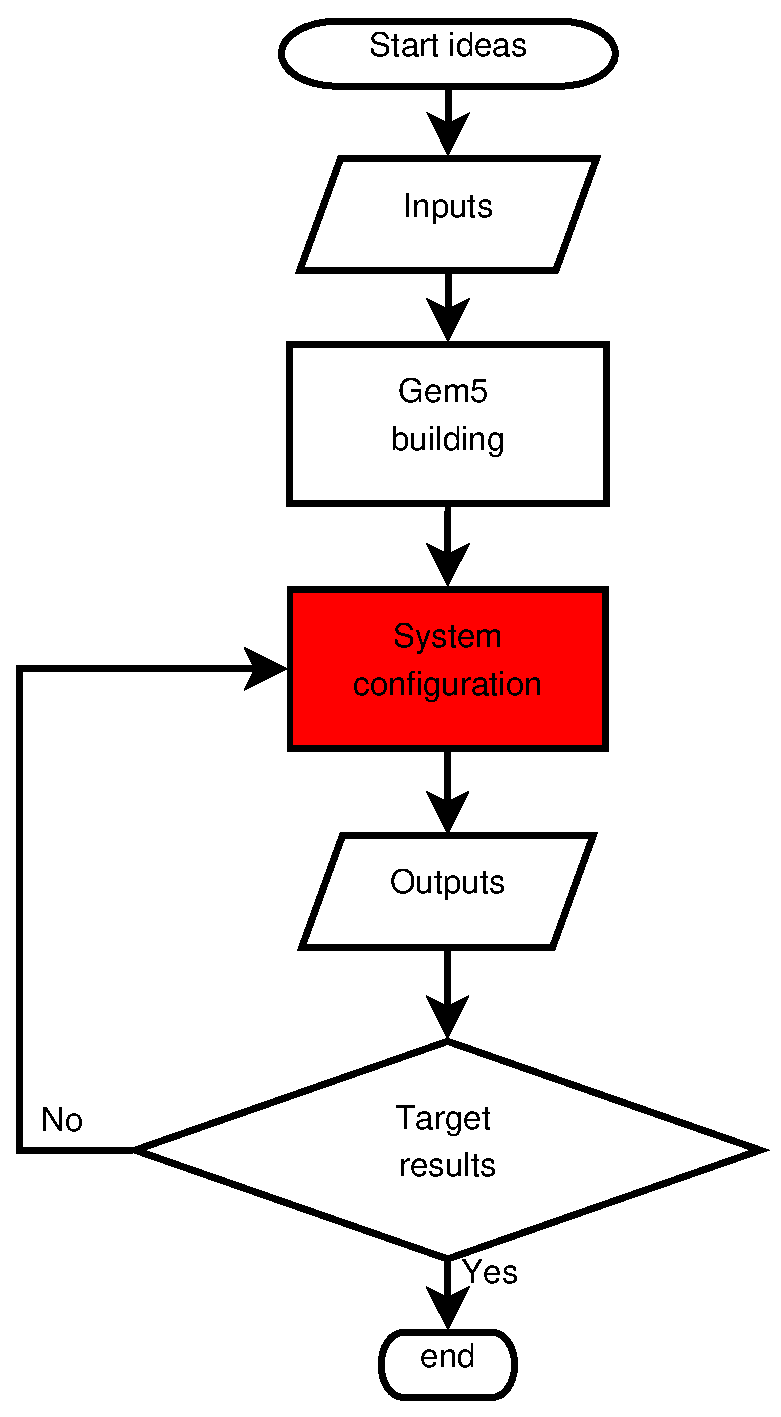
\includegraphics[width=0.3\linewidth]{methodofGarnetGem5Implementation}
	\caption{Phương pháp thực thi mô phỏng của đề tài}
	\label{fig:methodofGarnetGem5Implementation}
\end{figure}

\subsection{Kết quả mô phỏng thực nghiệm} \label{results}
Việc thực hiện mô phỏng thực nghiệm được dựa trên cơ sở các phân tích đã được nêu ra trong hình~\ref*{fig:methodofGarnetGem5Implementation} trang ~\pageref{fig:methodofGarnetGem5Implementation}

Sau khi thực hiện việc mô phỏng và kết quả đạt được với các điểm xác định bão hòa như hình trong bảng thống kê hình~\ref{fig:outputs_results} trang ~\pageref{fig:outputs_results}

\begin{figure}[h!]
	\centering
	\includegraphics[width=1\linewidth]{images/outputs_results}
	\caption{Kết quả mô phỏng khảo sát điểm làm việc bão hòa với thông số độ trễ trung bình gói tin trong mạng}
	\label{fig:outputs_results}
\end{figure}

\textbf{Nhận xét kết quả mô phỏng:}
Với kết quả thu được trong hình~\ref{fig:outputs_results}, một điểm chung ta có thể thấy rõ đối với hầu hết tất cả các benchmark đó chính là điểm bão hòa của mạng tại điểm IR xấp xỉ bằng 30\% tương đương với giá trị truyền vào mạng khi cấu hình là 0.3. Tuy nhiên, vẫn còn một số điểm bất thường cần khảo sát thêm với các kết quả đầu ra bởi thông số độ trễ truyền thông gói tin trung bình trong mạng là chưa xác định rõ được ví dụ như tại các điểm IR = \{0.8, 0.85\} của benchmark "\textit{shuffle}" hay IR = 0.9 của benchmark "\textit{reverse}" và được biểu diễn bằng ký hiệu "x". Một điểm có thể phát triển hướng đề tài là việc giải thích các điểm gây ra hiện tượng kết quả bất thường như trên có thể được đi sâu xem xét đến việc cấu hình mạng cũng như đặc trưng riêng của từng benchmark đối với hệ thống mạng trên chip garnet2.0 đang xét đến trong hệ thống này.
\subsection{Kết luận}\label{conclustion}
%%%%%%%%%%%%%%%%%%%%%%%%%%%
Như vậy với việc thực thi cài đặt bộ mô phỏng và khảo sát điểm bão hòa của thông số độ trễ truyền trung bình trong mạng trên chip tại các điểm tải tin xác định đã đạt được một số kết quả như sau:
\begin{itemize}
	\item Biết cách vận hành công cụ Gem5 để xây dựng các lõi vi xử lý tiên tiến như RISCV, X86, ARM, SPARC...
	\item Biết cách cấu hình và mô phỏng một hệ thống mạng trên chip (Garnet2.0) trên Gem5, là tiền đề, cơ sở để phát triển hướng nghiên cứu về sau.
	\item Khảo sát được điểm bão hòa của mạng trên chip với đầu ra khảo sát là độ trễ truyền thông tải tin trung bình trong mạng.
\end{itemize}

Tuy nhiên, còn tồn tại một số nhược điểm dưới đây:
\begin{itemize}
	\item Các kịch bản khảo sát chưa đủ lớn, chưa bao quát được tất cả các trường hợp sinh lỗi hệ thống.
	\item Một số điểm bất thường chưa tính toán được trễ truyền thông trung bình gói tin mà chưa tìm ra được nguyên nhân gây lỗi.
	\item Chưa cấu hình chạy với chế độ FS để có thể minh chứng được các kết quả mô phỏng có tính thuyết phục hơn.
\end{itemize}

Một số hướng nghiên cứu và phát triển của đề tài có thể xem xét đến đó là làm sao để cấu hình hệ thống chạy mô phỏng với nhiều benchmark hơn cũng như có thể chạy với chế độ FS; Bên cạnh đó cũng xây dựng được các mô hình kiến trúc NoC có khả năng chống lỗi, các thuật toán dò lỗi, sửa lỗi có thể áp dụng vào trong hệ thống để các kết quả có đóng góp ý nghĩa hơn về mặt khoa học và ứng dụng thực tiễn sẽ thiết thực hơn.
%%%%%%%%%%%%%%%%%%%%%%%%%%% 
%Reference	
	\newpage
	\bibliographystyle{ieeetr}
	\bibliography{MyLibrary}
	
\end{document}